\documentclass[]{article}
\usepackage[utf8]{inputenc}
\usepackage{amssymb}
\usepackage{amsmath}
\usepackage{graphicx}

\newcommand*{\poly}{\ensuremath{\mathbb{P}}}
\newcommand*{\real}{\ensuremath{\mathbb{R}}}
\newcommand*{\landau}{\ensuremath{\mathcal{O}}}

%opening
\title{ILIAS-Lernkontrollen und -Übungen}
\date{Sommersemester 2019}

\begin{document}

\maketitle

\begin{abstract}
Lösungen zu den ILIAS-Lernkontrollen und -Übungen zur Vorlesung "Numerische Mathematik f.d. Fachrichtung Informatik" im SoSe 2019
\end{abstract}

\section{Vorlesung 1}
\subsection{Lernkontrolle}
\begin{enumerate}
	\item Erklären sie den Aufbau einer normalisierten Gleitkommazahl
		\begin{itemize}
			\item Gleitkommazahl: $\textit{Basis} * \textit{Mantisse}^{\textit{Exponent}}$
			\item Basis: Meistens Zweierpotenz (2,8,16)
			\item Exponent: $e_{min} \leq e = e_{min} + \sum_{l=0}^{L_e - 1}c_l B^l \leq e_{min} + B^{L_e} - 1 := e_{max}$
			\item Mantisse: \begin{itemize}
				\item Entweder 0 oder $m = \sum_{l=1}^{L_m}a_l B^{-l}$
				\item $B^{-1} \leq |m| < 1$
			\end{itemize}
			\item Normalisierung: Mantisse beginnt immer mit einer 1, also $a_1 \neq 0$
		\end{itemize}
	\item Geben Sie die Definition der Maschinengenauigkeit an und erklären Sie, in welcher Weise die Mantissenlänge $L_m$ die relative Genauigkeit der Darstellung reeller Zahlen durch eine normalisierte Gleitpunktzahl bestimmt
		\begin{itemize}
			\item Maschinengenauigkeit $eps = \frac{B^{(1 - L_m)}}{2}$.
			\item Ist die Mantisse länger (also $L_m$ größer), so können mehr Nachkommastellen dargestellt werden, da $eps$ kleiner wird.
		\end{itemize}
	\item Beschreiben Sie den IEEE-Standard des Double Precision-Formats und erklären Sie, warum $1+eps$ die kleinste Zahl echt größer $1$ in $FL$ ist
		\begin{itemize}
			\item 64Bit für Gleitpunktdarstellung
				\begin{itemize}
					\item Basis $2$ fest
					\item 1Bit Vorzeichen
					\item 11Bit Exponent mit $e_{min} = -1022$
					\item 52Bit Mantisse
				\end{itemize}
			\item Darstellbare (pos.) Zahlen von $10^{-308}$ bis $10^{308}$
			\item Rel. Genauigkeit $eps = 2^{-52}$, circa 16 Nachkommastellen genau
			\item Jede Zahl $x$ mit $1 < x < 1+eps$ ist zu klein, es werden Nachkommastellen abgeschnitten
			\item Bei normalisierten GKZ ist die 1 fest, es können also mehr Bits für die Nachkommastellen der Mantisse genutzt werden und die Genauigkeit steigt auf $\frac{eps}{2}$
		\end{itemize}
	\item Nennen Sie mögliche Fehlerquellen der Eingabedaten eines numerischen Verfahrens und innerhalb des Verfahrens selbst beim Lösen eines mathematischen Problems und formulieren Sie die Fragestellungen, welche der Stabilität eines Verfahrens und der Kondition des Problems zugrunde liegen
		\begin{itemize}
			\item Eingabedaten-Fehler: Rundungsfehler, Messwertfehler
			\item Kondition: "Wie wirken sich Störungen der Eingabedaten auf das Resultat aus, unabhängig vom Algorithmus?"
			\item Verfahrens-Fehler: Rundungsfehler, Approximationsfehler (wenn das Verfahren von vornherein nicht genau arbeitet)
			\item Stabilität: "Wie stark wirken sich Störungen im Algorithmus auf das Ergebnis aus?"
		\end{itemize}
	\item Vollziehen Sie die Untersuchung und Deutung der \textit{Kondition der Summe zweier Zahlen} der Vorlesung nach, indem Sie auch das Phänomen der \textit{Auslöschung} erklären \\
	\\
		Kondition von $x+y$: Betrachte $x+\epsilon_x$ und $y+\epsilon_y$ als gestörte Eingabedaten von $x$ und $y$. \\
		Die absolute Abweichung von $(x+\epsilon_x) + (y+\epsilon_y)$ zu $x+y$ ist $Abw_{abs} = |((x+\epsilon_x) + (y+\epsilon_y)) - (x+y)|$. Die relative Abweichung ist $Abw_{rel} = \frac{Abw_{abs}}{|(x+y)|} \leq \epsilon \frac{|x|+|y|}{|x+y|}$ fpr ein kleines $\epsilon$. Das Problem ist an sich gut konditioniert, nur für $x \approx (-y)$ kann es zur Auslöschung kommen.\\
	\\
		Auslöschung: Bei der Subtraktion von zwei fast gleich großen GKZ (erste paar Nachkommastellen gleich) kann es
		passieren dass der Unterschied so klein ist, dass er durch die Maschinengenauigkeit beeinflusst wird. Die gleichen Stellen werden ausgelöscht und nur Stellen mit Rundungsfehler bleiben bestehen.\\
	Beispiel: $a = 2,345678$ und $b = 2,346789$, so ist $(b-a) = 0,001111$. Die niedrigwertigsten Stellen sind sehr anfällig für Rundungsfehler (z.B. aus vorherigen Berechnungen) und die höchsten (korrekten) Stellen löschen sich zu $0$ aus.
\end{enumerate}

\section{Vorlesung 2}
\subsection{Lernkontrolle}
	\begin{enumerate}
		\item Erklären Sie, wann genau und warum eine Zerlegung $A=LR$ für $A$ existiert und mit welchem Aufwand sich diese berechnen lässt.
			\begin{itemize}
				\item $A = LR$ existiert $\Leftrightarrow$ Jede Matrix $A_{[1:n,1:n]}$ ($n = 1...N$) ist regulär
				\item Eine LR-Zerlegung kann in O($\frac{1}{3} N^3$) errechnet werden
			\end{itemize}
		\item Geben Sie an, für welche spezielle Klasse von Matrizen $A$ auf jeden Fall eine Zerlegung $A=LR$ existiert.
			\begin{itemize}
				\item Für Matrizen die bereits die Form von $L$ oder $R$ haben (obere o. untere Dreiecksmatrizen)
			\end{itemize}
		\item Erklären Sie, wann genau und warum eine Zerlegung $PA=LR$ für $A$ existiert.
			\begin{itemize}
				\item $A$ regulär $\Rightarrow$ Es existiert eine Permutationsmatrix $P$ sodass für $PA$ die Bedingungen aus 1. gelten
				\item $P$ kann während der Berechnung von $L, R$ durch Spaltenpivotwahl berechnet werden
			\end{itemize}
		\item Beschreiben Sie, wie sich das lineare Gleichungssystem $Ax=b$ bei Kenntnis einer Zerlegung $PA=LR$ lösen lässt, und geben Sie den Aufwand der einzelnen Schritte an.
			\begin{enumerate}
				\item[1.] Löse $Ly = Pb$ durch Vorwärtssubstitution in O($\frac{1}{2} N^2$)
				\item[2.] Löse $Rx = y$ durch Rückwärtssubstitution in O($\frac{1}{2} N^2$)
				\item[  ] Dies benötigt $2 \times$O($\frac{1}{2} N^2$) $=$ O($N^2$) Operationen
			\end{enumerate}
		\item Erklären Sie, warum die Kenntnis der Inversen $A^{-1}$ gegenüber einer bekannten Zerlegung $PA = LR$ beim Lösen von $Ax = b$ keinen Vorteil darstellt.
			\begin{itemize}
				\item Da bei Kenntnis von $A^{-1}$ immer noch $A^{-1} b$ errechnet werden muss. Dies benötigt auch O($N^2$) Schritte
			\end{itemize}
	\end{enumerate}
\subsection{Übung}
	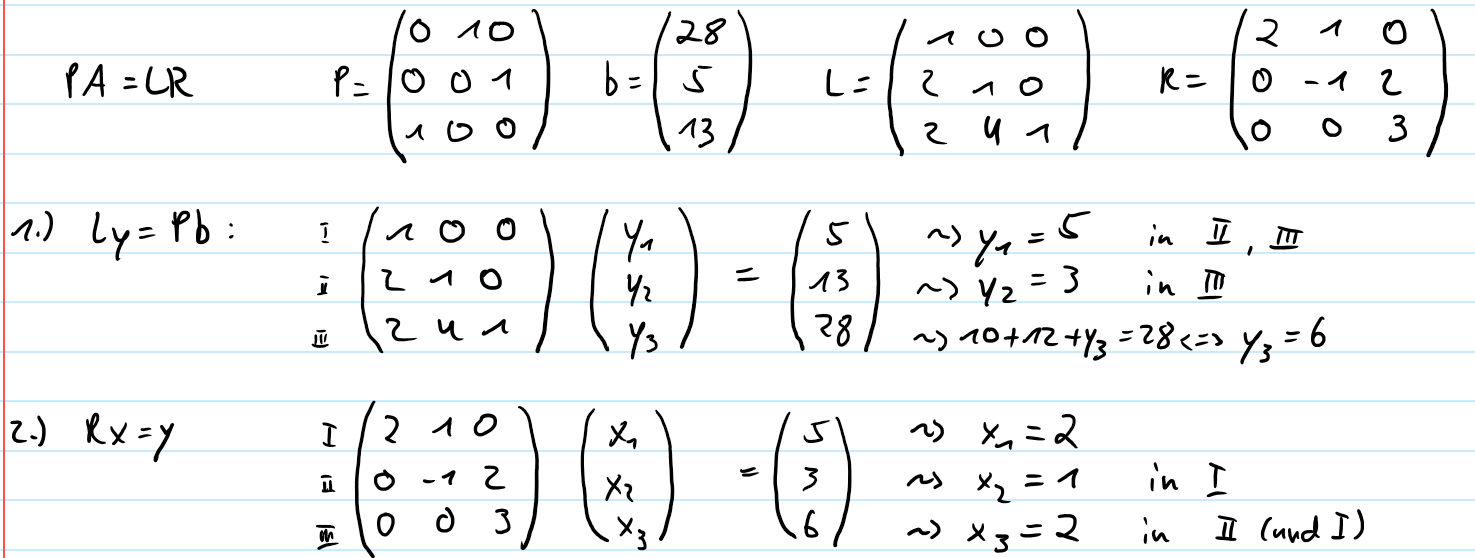
\includegraphics[width=\textwidth]{res/vl2-1.png}
	\\ \\
	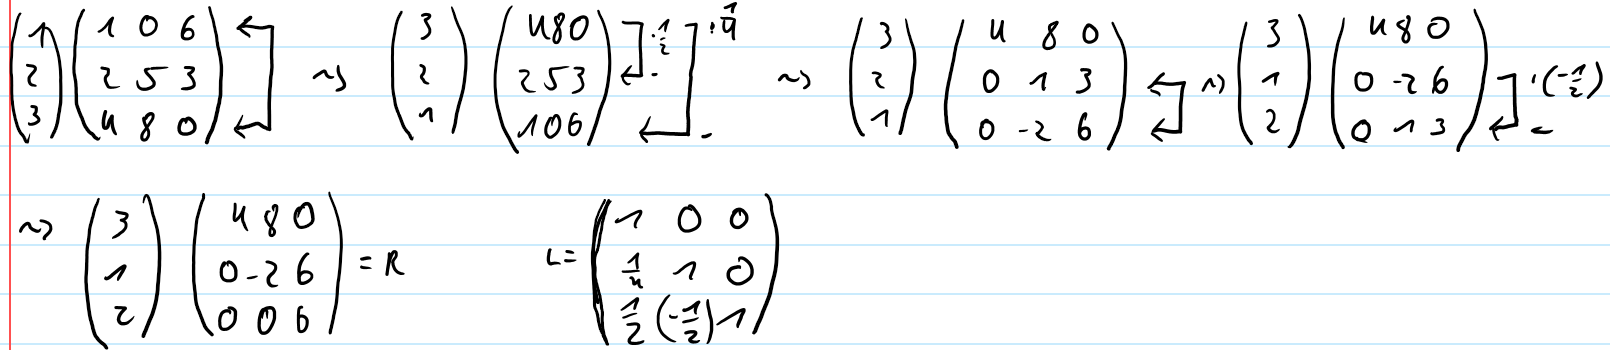
\includegraphics[width=\textwidth]{res/vl2-2.png}
		

\section{Vorlesung 3}
\subsection{Lernkontrolle}
	\begin{enumerate}
		\item Erklären Sie, für welche Matrizen $A$ genau eine Cholesky-Zerlegung existiert und wie bei Kenntnis einer solchen Zerlegung das Gleichungssystem $Ax=b$ gelöst werden kann.
			\begin{itemize}
				\item $A$ spd-Matrix $\Leftrightarrow$ Cholesky-Zerlegung $A=LL^T$ existiert
				\item Löse $Ax=b$ wie mit der LR-Zerlegung über Vorwärts- und Rückwärtssubstitition (anstelle von $R$ nehme $L^T$)
			\end{itemize}
		\item Geben Sie an, wie eine $QR$-Zerlegung einer Matrix $A \in \mathbb{R}^{M \times N}$ definiert ist, indem Sie die Faktoren beschreiben, und erklären Sie, wie sich ein lösbares LGS $Ax=b$ durch eine solche Zerlegung lösen lässt.
			\begin{itemize}
				\item $A=QR$ mit $Q \in \mathbb{R}^{M \times M}$ orthogonal (also $QQ^T = I_M$) und \\
				$R = \left (\begin{array}{r} \tilde{R} \\ 0 \end{array} \right)$ mit $\tilde{R} \in \mathbb{R}^{N \times N}$
				\item Eine $QR$-Zerlegung kann mit Householder-Transformationen errechnet werden
				\item Löse erst $Qc=b$ ($Q^{-1} = Q^T$, also $c = Q^Tb$)
				\item $Rx=c$ durch Rückwärtssubstitution
			\end{itemize}
		\item Nennen Sie einen Vorteil und einen Nachteil der $QR$-Zerlegung gegenüber der $LR$- und Cholesky-Zerlegung.
			\begin{itemize}
				\item Vorteil: Sehr stabiles Verfahren
				\item Nachteil: Mit O($\frac{2}{3} N^3$) am langsamsten
			\end{itemize}
		\item Wiederholen Sie Eigenschaften und die Struktur von Householder-Transformationen.
			\begin{itemize}
				\item Orthogonale Matrix $Q = I_M - 2w w^T$ mit $w \in \mathbb{R}^M, w^T w = 1$ sodass $Qv = \sigma e^1 = (\sigma$ $0 \dots 0)^T$ für ein $v \in \mathbb{R}^M, v \neq 0$
			\end{itemize}
		\item Erklären Sie, wie eine Householder-Transformation $Q$ effizient gespeichert werden kann und wie ein Produkt $Qy$ berechnet wird
			\begin{itemize}
				\item Die Householdervektoren $w_i$ können in $A$ gespeichert werden, für die $r_{nn}$ wird ein $N$-dim. Vektor benötigt
			\end{itemize}
	\end{enumerate}

\section{Vorlesung 4}
\subsection{Lernkontrolle}
	\begin{enumerate}
		\item Geben Sie zu einer Norm $|| * ||$ auf $\mathbb{R}^N$ die zugehörige Matrixnorm an und nennen Sie drei wichtige Beispiele solcher Normen.
			\begin{itemize}
				\item Allgemeine Matrixnorm $||A|| := sup_{x \neq 0} \frac{||Ax||}{||x||}$ für $A \in \mathbb{R}^{N \times N}$
				\item Zeilensummennorm $||A||_\infty$: $max_{m=1 \dots N} \sum_{n=1}^{N}|a_{nm}|$
				\item Spaltensummennorm $||A||_1$: $max_{m=1 \dots N} \sum_{n=1}^{N}|a_{mn}|$
				\item Spektralnorm $||A||_2$: $\sqrt{\textit{größter EW von }A^T A}$
			\end{itemize}
		\item Formulieren Sie die Frage, der sich die Kondition eines Problems widmet.
			\begin{itemize}
				\item "Wie wirken sich Störungen der Eingabegröße auf die Lösung aus, unabh. vom Algorithmus?"
			\end{itemize}
		\item Erklären Sie, was genau eine kleine Kondition bzw. eine große Kondition $cond(A)$ über das Problem $Ax=b$ aussagt.
			\begin{itemize}
				\item Die Kondition von $A$ ist die Sensitivität des rel. Fehlers von $A$ ggü. Störungen von $b$
				\item Eine kleine $cond(A)$ bedeutet geringe Sensitivität
			\end{itemize}
		\item Nennen Sie mindestens drei Eigenschaften der Funktion $cond(A)$
			\begin{itemize}
				\item $cond(A) = ||A||$ $||A^{-1}||$
				\item $cond(A) = cond(\lambda A),$ \quad $\lambda \in \mathbb{R} \backslash \{0\}$
				\item $cond(A) = \frac{max_{||y||=1}  ||Ay||}{min_{||x||=1} ||Ax||}$
			\end{itemize}
		\item Erklären Sie, warum die Kondition orthogonaler Matrizen bezüglich $||A||_2$ gleich 1 ist und wie sich die Kondition von symmetrischen und spd-Matrizen bezüglich dieser Norm berechnen lässt.  
			\begin{itemize}
				\item Da orthogonale Matrizen orthonormal bzgl. des Skalarprodutes sind
				\item $cond(A) = \frac{\textit{betragl. größter EW}}{\textit{betragl. kleinster EW}}$, wenn $A$ symm./spd.
			\end{itemize}
	\end{enumerate}
\subsection{Übung}
	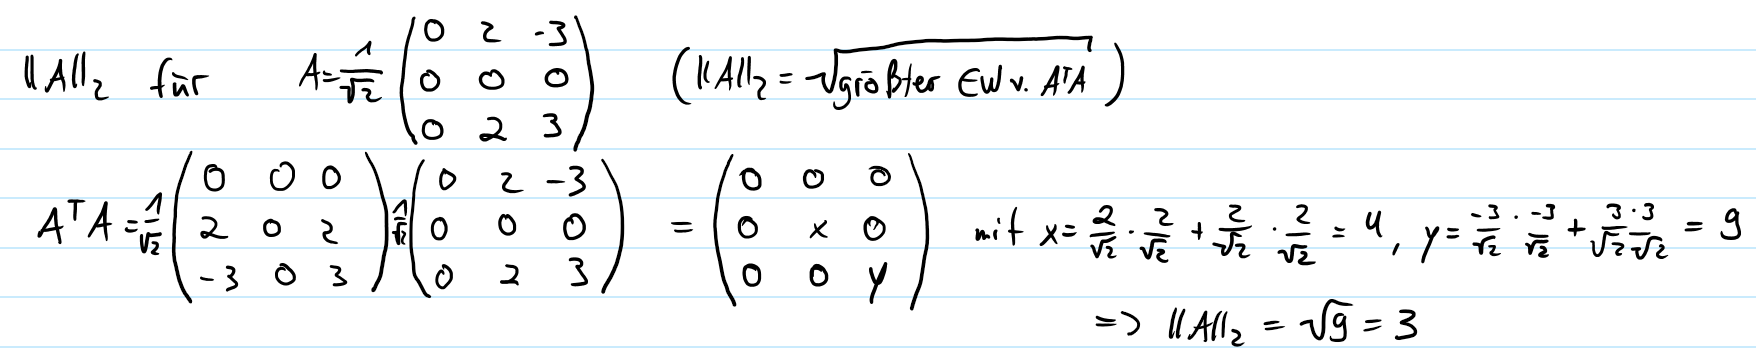
\includegraphics[width=\textwidth]{res/vl4-1.png}
	\\ \\
	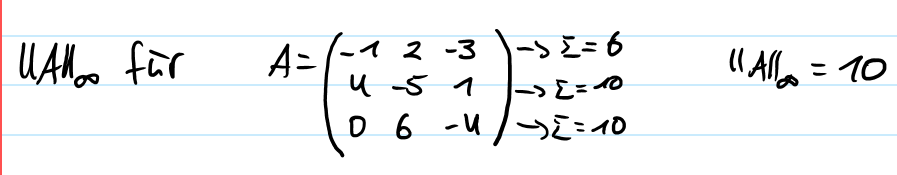
\includegraphics[width=\textwidth]{res/vl4-2.png}
	\\
	Die 1-Norm geht analog zur $\infty$-Norm nur mit den Spaltensummen.

\section{Vorlesung 5}
\subsection{Lernkontrolle}
	Betrachtet wird das lineare Ausgleichsproblem $||Ax-b|| = min!$ zu $A \in \mathbb{R}^{M \times N}, b \in \mathbb{R}^M$
	\begin{enumerate}
		\item Erklären Sie, in welcher Situation man ein solches lineares Ausgleichsproblem betrachtet.
			\begin{itemize}
				\item Im Fall $M > N$ ist $Ax=b$ überbestimmt und mglw. nicht lösbar
			\end{itemize}
		\item Beschreiben Sie den Zusammenhang des linearen Ausgleichsproblems mit der zugehörigen Normalengleichung und geben Sie diese an.
			\begin{itemize}
				\item Die Lösung $x$ für die Normalengleichung $A^TAx = A^Tb$ löst auch das Ausgleichsproblem
			\end{itemize}
		\item Erklären Sie, warum das lineare Ausgleichsproblem immer lösbar ist und unter welcher Bedingung an $A$ eine eindeutige Lösung vorliegt
			\begin{itemize}
				\item Die Normalengleichung ist immer lösbar (siehe Skript) $\Rightarrow$ Das lin. Ausgleichsproblem ist immer lösbar
				\item Ist $Rang(A)$ maximal, so ist $A^TA$ spd und das lin. Ausgleichsproblem ist eindeutig lösbar
			\end{itemize}
		\item Erklären Sie, wie und warum das lineare Ausgleichsproblem mit einer QR-Zerlegung von A gelöst werden kann.
			\begin{itemize}
				\item Sind $Q, R$ Matrizen aus der $QR$-Zerlegung mit $R = \left (\begin{array}{r} \tilde{R} \\ 0 \end{array} \right)$ mit $\tilde{R} \in \mathbb{R}^{N \times N}$, so ist $x = \tilde{R}^{-1} c$ mit $c$ aus $Q^Tb = \left (\begin{array}{r} c \\ d \end{array} \right)$ die Lösung des Ausgleichproblems
				\item Beweis siehe Skript S. 39 (gut zum Nachrechnen)
			\end{itemize}
		\item Erklären Sie, was eine Singulärwertzerlegung von $A$ mit $Rang(A) = R$ ist und wie diese genutzt werden kann, um eine Lösung des linearen Ausgleichsproblems mit minimaler euklidischer Norm zu bestimmen
			\begin{itemize}
				\item Singulärwertzerlegung von $A = U \Sigma V^T$ mit \\
				$U \in \mathbb{R}^{M \times M},V \in \mathbb{R}^{N \times N}$ orthogonal, \\
				$\Sigma = \left (\begin{array}{cc} \Sigma_R & 0 \\ 0&0 \end{array} \right) \in \mathbb{R}^{M \times N},$ \\ $\Sigma_R = diag(\sigma_1 \dots \sigma_R) \in \mathbb{R}^{R \times R}$
				\item bei $M>N$ ist $x = \sum_{r=1}^{R} \frac{(u^r)^Tb}{\sigma_r}v^r$ eine Lösung der Normalengleichung mit min. euklidischer Norm (siehe Übungen und ÜBs)
			\end{itemize}
	\end{enumerate}

\section{Vorlesung 6}
\subsection{Lernkontrolle}
	\begin{enumerate}
		\item Formulieren Sie das Newton-Verfahren zur Berechnung von $\sqrt{a}$ für $a  \in (1,4)$, indem Sie die Funktion $f$ und die Newton-Iteration explizit angeben, und erklären Sie, wie die Berechnung der Wurzel einer normierten Binärzahl $(1+m)2^e$ darauf zurückgeführt werden kann
			\begin{itemize}
				\item $f(x) = x^2 - a \Rightarrow x = \sqrt{a}$
				\item $2x_kd_k = -x^2 + a \Leftrightarrow 2 d_k = \frac{{x_k}^2}{x_k}+\frac{a}{x_k} \Leftrightarrow d_k = \frac{1}{2}({x_k} + \frac{a}{x_k})$
			\end{itemize}
		\item Geben Sie die allgemeine Newton-Iteration zur Nullstellengleichung $f(x)=0$ einer Funktion $f: \mathbb{R}^N \rightarrow \mathbb{R}^N$ an.
			\begin{itemize}
				\item $f'(x_k)d_k = -f(x_k)$
				\item $x_{k+1} = x_k + d_k$
			\end{itemize}
		\item Nennen Sie zwei wichtige Aspekte im Hinblick auf die Konvergenz des Newton-Verfahrens.
			\begin{itemize}
				\item Das Newton-Verfahren konvergiert lokal quadratisch
				\item Das Newton-Verfahren konvergiert nur bei guter Wahl von $x_0$, sonst kann es divergieren
			\end{itemize}	
		\item Erklären Sie die geometrische Deutung des Newton-Verfahrens im Fall $N=1$
			\begin{itemize}
				\item Das Newton-Verfahren legt im ersten Schritt eine Tangente an $f$ mit Nullstelle $x_0$ an
				\item In den darauffolgenden Schritten wird die Nullstelle der neuen Tangente der Berührungspunkt der alten Tangente mit $f$ 
			\end{itemize}
		\item Erklären Sie, was mit dem Vereinfachten Newton-Verfahren gemeint ist und was die Vereinfachung für Konsequenzen hat.
			\begin{itemize}
				\item Das berechnen von $f'(x_k)$ in $d_k f'(x_k) = -f(x_k)$ ist sehr kompliziert, da im mehrdim. Fall eine Jacobimatrix berechnetw erden muss
				\item Beim vereinfachten Newton-Verfahren wird anstelle von $f'(x_k)$ immer die Matrix $A \approx f'(x_0)$ genommen, also $d_k A = -f(x_k)$
				\item Die Konvergenz des Verfahrens wird dann linear anstelle von quadratisch
				\item Für die Matrix $A$ kann im ersten Schritt eine LR-Zerlegung errechnet werden, welche dann immer weiter genutzt werden kann
			\end{itemize}	
	\end{enumerate}
\subsection{Übung}
	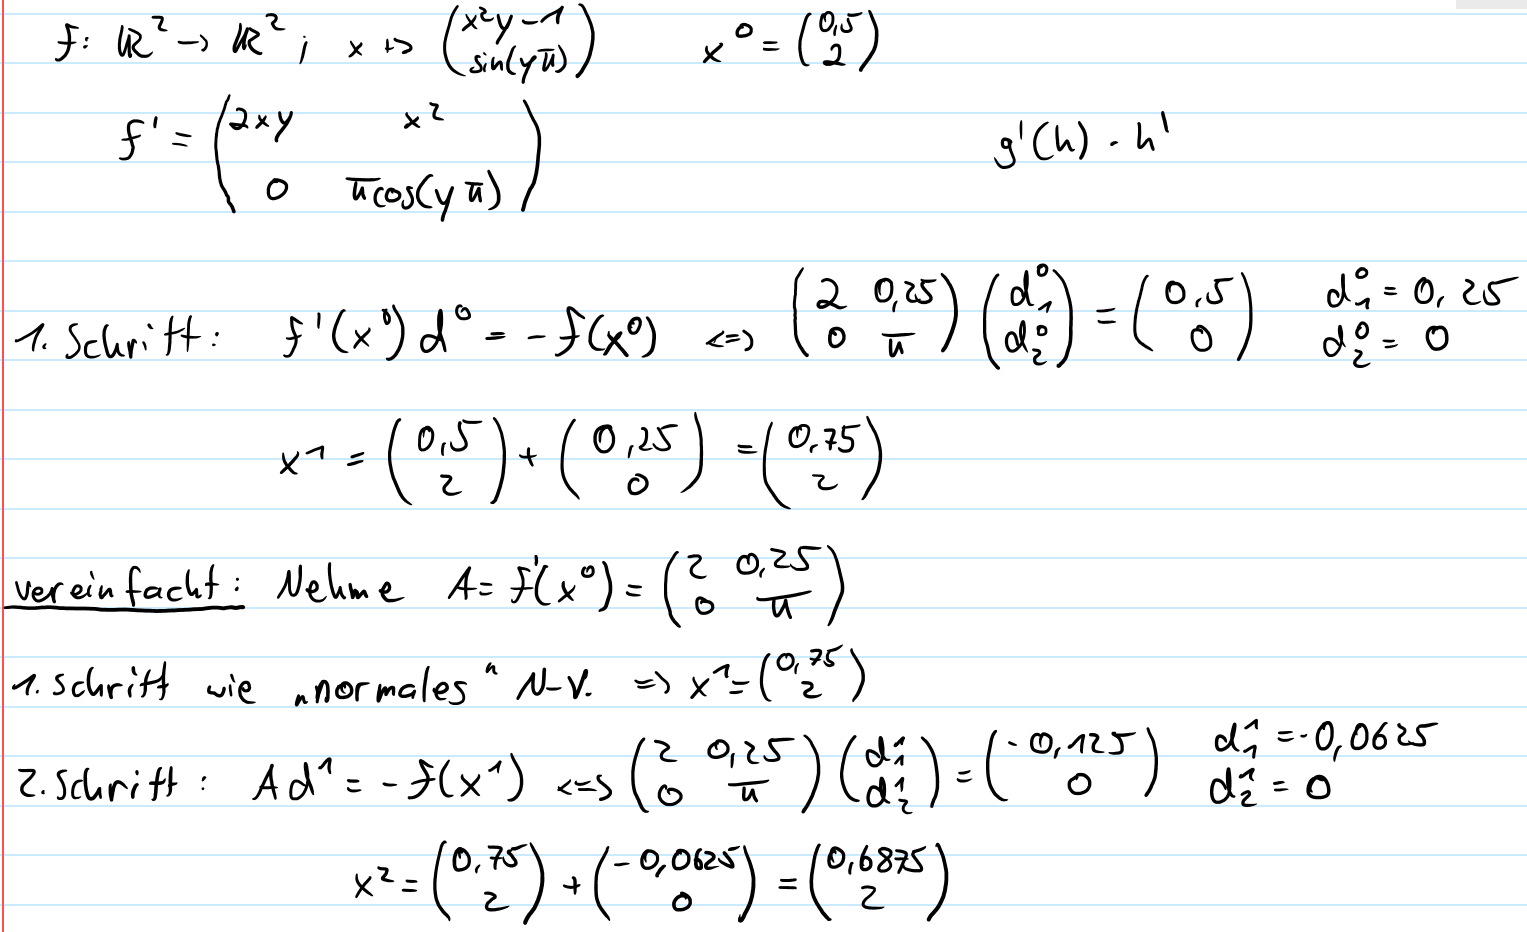
\includegraphics[width=\textwidth]{res/vl6-1.png}	

\section{Vorlesung 7}
\subsection{Lernkontrolle}
	\begin{enumerate}
		\item Formulieren Sie die Fragestellung der Polynominterpolation.
			\begin{itemize}
				\item Gegeben sind $N+1$ paarw. verschiedene Stützstellen $(x_0, f(x_0)), \dots (x_N, f(x_N))$
				\item Wir suchen ein Polynom $p$ mit $deg(p) \leq N$ mit $p(x_i) = f(x_i)$ für alle $i \in (0, N)$
			\end{itemize}
		\item Begründen Sie, warum das Problem der Polynominterpolation eine eindeutige Lösung besitzt
			\begin{itemize}
				\item Ein Polynom $p$ mit $deg(p) \leq N$ ist durch $N+1$ Stützstellen exakt definiert
				\item Bsp.: Eine Gerade aus $\mathbb{P}_1$ ist durch 2 Punkte exakt definiert
			\end{itemize}	
		\item Vollziehen Sie nach, welche Größe als Maß für die Kondition des Problems gilt und warum Interpolationspolynome von hohem Grad zumindest bei äquidistanten Stützstellen mit Vorsicht zu genießen sind.
			\begin{itemize}
				\item Das Maß für die Kondition der Interpolation ist die Lebesque-Konstante: $\Lambda_N := max_{x \in [a,b]} \sum_{n=0}^N |L_n(x)|$
				\item Die Lebesque-Konstante misst die Auswirkung von Störungen der Stützstellen $(x_0, \tilde{f}(x_0)), \dots (x_N, \tilde{f}(x_N))$ und dem gestörten Interpolationspolynom $\tilde{p}$
				\item $|p(x) - \tilde{p}(x)| = |\sum (f_n - \tilde{f}_n) L_n(x)| \\
					\leq \sum |(f_n - \tilde{f}_n)| |L_n(x)| \\
					\leq max_{n=0 \dots N} |(f_n - \tilde{f}_n)| \sum |L_n(x)|$
				\item Bei Polynomen mit hohem Grad und äquidistanten Stützstellen wächst $\Lambda_N$ sehr stark an	 
			\end{itemize}
		\item Geben Sie die Newton-Darstellung des Interpolationspolynoms an und vergleichen Sie diese mit der Lagrange-Darstellung.
			\begin{itemize}
				\item Bei der Newton-Darstellung wird versucht, das Interpolationspolynom schrittweise aus Polynomen mit niedrigerem Grad aufzubauen
				\item Newton-Darstellung: $p_{0,N}(x) = a_0 + a_1(x - x_0) + a_2(x - x_0)(x - x_1) + \dots + a_N(x-x_0) \cdot \dots \cdot (x-x_{N-1})$
				\item Lagrange-Darstellung: $p(x) = \sum_{n=0}^{N} f_n L_n(x)$ mit $L_n(x) = \prod_{m=0, m \neq n}^{N} \frac{x-x_m}{x_n - x_m}$
			\end{itemize}
		\item Formulieren Sie das Lemma von Aitken und erklären Sie, wie daraus die Formel für die dividierten Differenzen hergeleitet werden kann.
			\begin{itemize}
				\item Das Lemma besagt, dass die Interpolationspolynome rekursiv aufgebaut werden können
				\item Die Leitkoeffizieniten der Rekursion des Lemmas sind $f_{n,k} = \frac{f_{n,k-1} - f_{n+1,k}}{x_n - x_k}$
			\end{itemize}
	\end{enumerate}

\section{Vorlesung 8}
\subsection{Lernkontrolle}
	\begin{enumerate}
		\item Wiederholen Sie das Restglied der Polynominterpolation, um den Interpolationsfehler $f(x)-p(x)$ für eine hinreichend glatte Funktion $f: [a,b]\rightarrow \mathbb{R}$ anzugeben. 
			\begin{itemize}
				\item $f(x) - p(x) = (x-x_0) \cdot \dots \cdot (x-x_{N}) \frac{f^{N+1}(\tilde{x})}{(N+1)!}$ wobei $\tilde{x}$ eine Zwischenstelle zu $x$ ist
			\end{itemize}
		\item Formulieren Sie die beiden Definitionen der Tschebyscheff-Polynome und geben Sie vier Eigenschaften dieser Polynome an
			\begin{itemize}
				\item Rekursiv: $T_0(x) = 1, T_1(x) = x, T_{n+1}(x) = 2x \cdot T_n(x) - T_{n-1}(x)$
				\item Alternativ: $T_n(x) = cos(n \cdot arccos(x))$
				\item 4 Eigenschaften:
				\begin{itemize}
					\item Stehen alle im Skript auf S.58 wer lust die abzutippen kann gerne ein PR aufmachen %TODO
				\end{itemize}
			\end{itemize}
		\item Nennen Sie zwei Gründe, warum Tschebyscheff-Stützstellen eine gute Wahl an Stützstellen sind, und geben Sie die Tschebyscheff-Stützstellen an
			\begin{itemize}
				\item Unter allen Stützstellen wird $(x-x_0) \cdot \dots \cdot (x-x_{N})$ minimal wenn die $x_n$ genau die Nullstellen des $(N+1)$-ten Tschebyscheff-Polynomes sind
				\item Die Lebesque-Konstante $\Lambda_N$ ist bei Tschebyscheff-Stützstellen geringer als bei äquidistanten Stützstellen
				\item Die Nullstellen und damit die $x_n$ sind leicht berechenbar: $x_n = cos(\frac{2n+1}{2N+2} \pi)$
			\end{itemize}
		\item Erklären Sie, wie und warum sich die Koeffizienten der Tschebyscheff-Darstellung des Interpolationspolynoms berechnen lassen
			\begin{itemize}
				\item Die Tschbyscheff-Polynome $T_{0\dots N}$ bilden eine Basis von $\poly_N$, da sie orthogonal bzgl. des Skalarprodutes sind
				\item $p(x) = \frac{1}{2}c_o + c_1T_1(x) + \dots + c_NT_N(x)$ mit \\
					$c_n = \frac{2}{N+1} \sum_{m=0}^{N} f_m cos(n \cdot \frac{2n+1}{2N+2} \pi)$
			\end{itemize}
		\item Geben Sie die Berechnungsvorschrift des (stabilen) Clenshaw-Algorithmus an, mit dem das Interpolationspolynom $p(x) = \frac{1}{2}c_o + c_1T_1(x) + \dots + c_NT_N(x)$ an der Stelle $x$ ausgewertet werden kann.
			\begin{itemize}
				\item Mit $d_{N+2} = d_{N+1} = 0, d_n = c_n + 2x \cdot d_{n+1} - d_{n+2}$ gilt: \\
				$p(x) = \frac{1}{2}(d_0 - d_2)$
			\end{itemize}		
	\end{enumerate}

\section{Vorlesung 9}
\subsection{Lernkontrolle}
	Ein kubischer Spline ist eine $C^2$-Funktion $s: [a,b] \rightarrow \real$, welche die Stützpunkite $(x_0, f(x_0)), \cdots (x_N, f(x_N))$ interpoliert, wobei jedes $s_n \in \poly_3$ liegt.
	\begin{enumerate}
		\item Formulieren Sie die Definition dreier unterschiedlicher Klassen von interpolierenden kubischen Splines und geben Sie eine Minimalitätseigenschaft dieser Splines an, welche insbesondere Oszillationen [...] verhindert.
			\begin{itemize}
				\item Drei Klassen:
					\begin{itemize}
						\item Eingespannt: $s'(a) = v_0, s'(b)=v_n$ für vorgeg. $v_0, v_n$
						\item Natürlich: $s''(a)=s''(b)=0$
						\item Periodisch: $s'(a)=s'(b)$ und $s''(a)=s''(b)$
					\end{itemize}
				\item Minimalitätseigenschaft: $\int_a^b |s''(x)|^2 dx$ minimal
			\end{itemize}
		\item Geben Sie den Ansatz für $s_n$ an und erklären Sie diesen
			\begin{itemize}
				\item $s_n \in \poly_3$ besteht aus interpolierendem und glättendem Anteil
				\item $s_n(x) = y_{n-1} + (x - x_{n-1}) y_{n-1, n}$ $ + $  \\
								$(x - x_{n-1})( x - x_n) ( \alpha_n (x - x_{n-1}) + \beta_n (x - x_n) ) $
				\item Ausserdem: $s_n(x_{n-1}) = f(x_{n-1})$ und $s_n(x_n) = f(x_n)$				
			\end{itemize}	
		\item Vollziehen Sie nach, warum durch die Def. $\gamma_{n-1} = s_n ''(x_{n-1})$ und $ \gamma_n = s_n ''(x_n)$ bereits $N-1$ Glattheitsbedingungen automatisch erfüllt sind und geben Sie die übrigen $N-1$ Glattheitsbedingungen an
			\begin{itemize}
				\item Die Def. sind $2N$ Gleichungen für $N+1$ Unbekannte ($\gamma_0, \dots \gamma_N$). Dadurch sind $N-1$ Glattheitsbed. an die zweite Ableitung direkt erfüllt
				\item Die Bedigungen an die erste Ableitung $s_n'(x_n) = s_{n+1}(x_n)$ für $n=1, \dots , N-1$ sind die anderen $N-1$ Bedingungen
			\end{itemize}
		\item Geben Sie das LGS zur Bestimmung von $(\gamma_0, \dots , \gamma_N)^T$ im Fall äquidistanter Stützstellen $(h_n = h)$ für eingespannte Splines an
			\begin{itemize}
				\item Skript S. 70 unten, wer das abtippen will kann gerne ein PR aufmachen %TODO
			\end{itemize}
		\item Sei $s(x)$ der eingespannte kubische Spline zu den Stützstellen oben und $\tilde{s}(x)$ entsprechend zu den gestörten Werten $\tilde{f}(x)$ für $n = 0, \dots , N$ Erklären Sie, wie die "Lagrange"-Splines $l_n(x)$ definiert sind und wie und warum sich damit die Differenz $s(x) - \tilde{s}(x)$ darstellen lässt
			\begin{itemize}
				\item Lagrange-Splines: $l_n(x_m) = \begin{cases} 1 & n = m \\0 & \text{sonst} \end{cases}$
				\item $|s(x) - \tilde{s}(x)| \leq \sum |y_n - \tilde{y}_n| |l_n(x)| \leq \sum |l_n(x)| \cdot ( max_{n=0\dots N} |y_n - \tilde{y}_n| ) \leq \Lambda_N \cdot ( max_{n=0\dots N} |y_n - \tilde{y}_n| )$ wobei $y_i = f(x_i)$
			\end{itemize}
	\end{enumerate}	

\section{Vorlesung 10}
\subsection{Lernkontrolle}
	\begin{enumerate}
		\item Geben Sie die allgemeine Form einer Quadraturformel zur Approximation von $\int_b^a f(x) dx$ an und benennen Sie auftretende Größen
			\begin{itemize}
				\item $(b-a) \sum b_k \cdot f(a + c_k(b-a))$
					\begin{itemize}
						\item[$\rightarrow$] $b_k$ Gewichte, $c_k$ Knoten/Stützstellen
					\end{itemize}	
			\end{itemize}
		\item Wiederholen Sie die Definition der Ordnung $p$ einer Quadraturformel und vollziehen Sie die Herleitung der Ordnungsbedingungen nach
			\begin{itemize}
				\item Eine Quadraturformel hat Ordnung $p$ wenn sie Polynome in $\poly_{p-1}$ exakt integiert, aber Polynome in $\poly_p$ nicht mehr
				\item QF hat Ordnung $p \Leftrightarrow \frac{1}{q} = \sum b_k \cdot c_k^{(q-1)}$ für $q = 1, \dots , p$ aber nicht mehr für $q = (p+1)$
			\end{itemize}
		\item Vollziehen Sie die Begründung nach, dass bei Vorgabe der Knoten $c_1, \dots , c_s$ und der Forderung $p \geq s$ die Gewichte $b_1, \dots , b_s$ eindeutig bestimmt sind
			\begin{itemize}
				\item Mit allen Ordnungsbedingungen aus 2. wird ein LGS der Dimension $s$ erstellt, welches nur die Unbekannten $b_1, \dots , b_s$ enthält. Dieses LGS kann (zB mit der LR-Zerlegung) gelöst werden.
			\end{itemize}
		\item Geben Sie die Definition einer symmetrischen Quadraturformel an und treffen Sie eine Aussage im Hinblick auf die Ordnung solcher Formeln.
			\begin{itemize}
				\item Bei einer symmetrischen QF sind die Knoten $c_i$ symm. zum Punkt $\frac{1}{2}$ verteilt
					\begin{itemize}
						\item[$\rightarrow$] $c_k = 1 - c_{s+1-k}$
						\item[$\rightarrow$] $b_k = b_{s+1-k}$
					\end{itemize}
				\item Die Ordnung einer symm. QF ist gerade	
			\end{itemize}
		\item Nennen Sie Beispiele von Quadraturformeln, erklären Sie jeweils die Approximationsidee, geben Sie jeweils die Knoten, Gewichte und die Ordnung an und klassifizieren Sie in symmetrisch und nicht symmetrisch.
			\begin{itemize}
				\item Rechteckformel
					\begin{itemize}
						\item $f$ wird durch ein Rechteck der Höhe $f(a)$ approximiert
						\item $b_1 = 1, c_1 = 0$
						\item Ordnung $p = 1$
					\end{itemize}
				\item Mittelpunktformel
					\begin{itemize}
						\item $f$ wird durch ein Rechteck der Höhe $f(a + \frac{b+a}{2})$ approximiert
						\item $b_1 = 1, c_1 = 0$
						\item Ordnung $p = 2$
					\end{itemize}
				\item Trapezformel
					\begin{itemize}
						\item $f$ wird durch ein Trapez von $f(a)$ nach $f(b)$ approximiert
						\item $b_1 = b_2 = \frac{1}{2}, c_1 = 0, c_2 = 1$
						\item Ordnung $p = 2$
					\end{itemize}
				\item Simpsonformel
					\begin{itemize}
						\item $f$ wird durch eine Parabel durch die 3 Punkte $f(a), f(\frac{a+b}{2}), f(b)$ approximiert
						\item $b_1 = b_3 = \frac{1}{6}, b_2 = \frac{4}{6}, c_1 = 0, c_2 = \frac{1}{2}, c_3 = 1$
						\item Ordnung $p = 4$
					\end{itemize}
			\end{itemize}
	\end{enumerate}

\section{Vorlesung 11}
\subsection{Lernkontrolle}
	\begin{enumerate}
		\item Vollziehen Sie den Ansatz zur Bestimmung von Quadraturformeln erhöhter Ordnung nach
			\begin{itemize}
				\item Muss noch dringend nachgetragen werden! %TODO
			\end{itemize}
		\item Begründen Sie damit, welche maximale Ordnung eine Quadraturformel besitzen kann
			\begin{itemize}
				\item Die max. Ordnung einer QF ist $2s$
			\end{itemize}
		\item Nennen Sie die Gewichte und Knoten der Quadraturformel mit maximaler Ordnung und nennen Sie zwei Eigenschaften dieser Formeln
			\begin{itemize}
				\item Solche Formeln haben Grad $2s$ und heißen Gauß-Quadraturformeln
				\item $c_k = \frac{1}{2}(1 + \gamma_k), \gamma_k$ sind die Nullstellen des Legrende-Polynomes vom Grad $s$. Die $b_k$ können mit den Ordnungsbedingungen errechnet werden.
				\item Die Gewichte sind alle positiv
				\item Die Formel ist symmetrisch
			\end{itemize}
		\item Vollziehen Sie nach, warum das Funktional $R$ bei der Untersuchung des Quadraturfehlers auftritt und geben Sie die Darstellung von Peano für $R(g)$ für $g \in C^p([a,b], \real)$ ohne die genaue Formel des Peano-Kerns an
			\begin{itemize}
				\item Warum tritt R auf? %TODO
				\item $R(g) = \int_0^1 K_q(t) g^{(q)}(t) dt$, wobei $K_q(t)$ der Peano-Kern ist
			\end{itemize}
		\item Formulieren Sie den Quadraturfehler auf dem Intervall $[a,b]$ und bei Anwendung einer summierten Quadraturformel (jeweils QF auf Teilintervall angewendet) zur Zerlegung $a = x_0 < \dots < x_N = b$ auf dem Gesamtintervall
			\begin{itemize}
				\item Fehler auf $[a,b]$: \\
						$( \int_a^b f(x) dx ) - ( (b-a)\sum b_k \cdot f(a+c_k(b-a)))$
				\item Fehler wenn $[a,b]$ auf $N$ Teilintervalle mit jeweiliger Länge $h_i$ aufgeteilt wurde: \\
						$( \int_a^b f(x) dx ) - ( \sum_{i=1}^N h_i \sum_{k=1}^s b_k \cdot f(x_{n-1} + c_k h_n )$ 
			\end{itemize}
	\end{enumerate}

\section{Vorlesung 12}
\subsection{Lernkontrolle}
	\begin{enumerate}
		\item Geben Sie die definierende Gleichung für Eigenwerte und Eigenvektoren an und erklären Sie, warum die Eigenwerte die Nullstellen des charakteristischen Polynoms sind, jedoch nicht über dieses berechnet werden sollten
			\begin{itemize}
				\item Eigenwert-Eigenvektor-Gleichung: $Av = \lambda v, A \in \real^{N \times N}, v \in \real^N, \lambda \in \real$
				\item Berechnung über Nullstellen des char. Polynoms möglich, da $Av = \lambda v  \Leftrightarrow (A- \lambda I_N)v = 0$
				\item Nullstellengleichung bei Polynomen sehr schlecht konditioniert
			\end{itemize}
		\item Geben Sie die Konditionszahl eines einfachen Eigenwerts der Matrix $A \in \real^{N \times N}$ an und definieren Sie dabei auftretende Größen. Warum ist der minimale Wert der Konditionszahl größer gleich $1$?
			\begin{itemize}
				\item Gestörte Matrix $\tilde{A}$ mit $\tilde{a_{mn}} = a_{mn}(1 + \epsilon_{mn})$ wobei $|\epsilon| \leq eps$
				\item Anders: $\tilde{A} = A + eps\cdot C$ mit $|c_{mn}| \leq |a_{mn}|$. Es sei $A(\epsilon) = A + \epsilon \cdot C$
				%\item $\lambda(\epsilon) = \lambda + \epsilon \frac{u^T C v}{u^T v} + \mathcal{O}(\epsilon^2)$
				\item $\frac{1}{|u^Tv|}$ mit $Av = \lambda v, u^TA = \lambda u^T, ||v||_2 = ||u||_2 = 1$ ist Konditionszahl zu $\lambda$
			\end{itemize}
		\item Formulieren Sie die Hauptidee der Vektoriteration, indem Sie insbesondere die nötigen Voraussetzungen an die Matrix $A$ angeben und erklären, wie sich damit ein Eigenwert von $A$ berechnen lässt.
			\begin{itemize}
				\item Vektoriteration findet betragsmäßig größten einfachen Eigenwert (hier immer $\lambda_1$)
				\item Matrix $A$ muss also folgende EWs haben: $|\lambda_1| > |\lambda_2| \geq \dots \geq |\lambda_N|$
				\item Wähle $x^0 = \mu_1v^1 + \dots + \mu_nv^N$ und berechne $Ax^0 = \mu_1\lambda_1v^1 + \dots + \mu_n\lambda_Nv^N = \lambda_1 ( \mu_1v^1 + \frac{\lambda_2}{\lambda_1}\mu_2v^2 + \dots)$
				\item Alle Werte ausser $v^1$ werden um $\lambda_1$ gedämpft
				\item Diese Multiplkation wird $k$-mal wiederholt: $A^kx^0 = \lambda_1^k ( \mu_1v^1 + (\frac{\lambda_2}{\lambda_1})^k \mu_2v^2 + \dots)$
				\item Das ganze konvergiert gegen $\mu_1v^1$, wenn $\mu_1 \neq 0$ und muss nur noch nach jedem Schritt normiert werden
			\end{itemize}
		\item Formulieren Sie die Hauptidee der Inversen Vektoriteration, indem Sie insbesondere die nötigen Voraussetzungen an die Matrix $A$ angeben und erklären, wie sich damit ein Eigenwert von A berechnen lässt
			\begin{itemize}
				\item $A \in \real^{N \times N}$ symmetrisch mit einem betragmäßig kleinsten EW nahe $0$
				\item $A$ ist durch die Voraussetzungen regulär, also ex. $A^{-1}$ mit EWs $\frac{1}{\lambda_i}$. Der kleinste EW von $A$ wird also zum größten EW von $A^{-1}$
				\item Es wird iterativ berechnet: $y^k = \frac{x^k}{||x^k||_2}$ und $Ax^{k+1} = y^k$. Also 1 LGS pro Schritt
			\end{itemize}
		\item Formulieren Sie die Problemstelllung der Spektralen Bisektion.
			\begin{itemize}
				\item Sei $(V,E)$ ein ungerichteter, zusammenhängender Graph
				\item Finde Zerteilung in 2 Mengen, sodass beide Mengen ungefähr gleich viele Knoten enthalten
			\end{itemize}
	\end{enumerate}

\section{Vorlesung 13}
\subsection{Lernkontrolle}
	\begin{enumerate}
		\item Formulieren Sie den QR-Algorithmus zur Berechnung der Eigenwerte einer Matrix $A \in \real^{N \times N}$, welche nur reelle Eigenwerte mit $|\lambda_1| > \dots > |\lambda_N|$ besitzt
			\begin{enumerate}
				\item Setze $A_0 = A$ und $k = 0$
				\item Zerlege $A_k = Q_kR_k$ mittels QR-Zerlegung
				\item Berechne $A_{k+1} = R_kQ_k$ und $k = k+1$ und zurück zu 2.
			\end{enumerate}
			\begin{itemize}
				\item $A_k$ konvergiert gegen obere rechte Dreicksmatrix $R$ mit EWs auf der Hauptdiagonalen
			\end{itemize}
		\item Vollziehen Sie nach, wie $A$ durch $N-2$ Householder-Transformationen auf Hessenbergform gebracht werden kann
			\begin{itemize}
				\item $Q^TAQ = H$ mit $Q = Q_1 \cdots Q_{N-2}$, wobei $Q_i$ eine Householder-Transformation ist
			\end{itemize}
		\item Formulieren Sie den QR-Algorithmus mit Shift und erklären Sie, warum der Aufwand (unabhängig vom Shift) pro Iterationsschritt $\landau(N^2)$ Operationen beträgt
			\begin{enumerate}
				\item Setze $H_0 = H$ und $k = 0$
				\item Zerlege $H_k - \mu_kI_N = Q_kR_k$ mittels QR-Zerlegung
				\item Berechne $H_{k+1} = R_kQ_k + \mu_kI_N$ und $k = k+1$ und zurück zu 2.
			\end{enumerate}
			\begin{itemize}
				\item Beim QR-Algorithmus mit Shift wird $A$ erst in Hessenbergform gebracht, was den Aufwand der QR-Zerlegung auf $\landau(N^2)$ reduziert
			\end{itemize}
		\item Erklären Sie, wie sich die Symmetrie in der Ausgangsmatrtix $A$ in der Struktur der $H_k$ widerspiegelt, und denken Sie kurz darüber nach, wie sich diese Struktur auf die Anzahl an Operationen auswirkt
			\begin{itemize}
				\item Ist $A$ symmetrisch, so ist $H$ eine Tridiagonalmatrix
				\item Der Aufwand der Transformationen wird von $\frac{5}{3}N^3$ auf $\frac{2}{3}N^3$ reduziert
			\end{itemize}
		\item Erklären Sie grob, was quadratische bzw. im Fall einer symmetrischen Matrix kubische Konvergenz bei der Shiftwahl $\mu_k = h_{NN}^{(k)}$ bedeutet
			\begin{itemize}
				\item Kann noch nachgetragen werden %TODO
			\end{itemize}
	\end{enumerate}

\section{Vorlesung 14}
\subsection{Lernkontrolle}
	\begin{enumerate}
		\item Formulieren Sie typische Eigenschaften der Matrix $A \in \real^{N \times N}$ bzw. Anforderungen an die Lösung $x_*$, bei denen das LGS $Ax = b$ iterativ gelöst werden kann/sollte
			\begin{itemize}
				\item $N$ ist sehr groß oder $A$ ist sehr dünn besetzt
				\item Es wird nur eine Approximation von $x_*$ benötigt
			\end{itemize}
		\item Formulieren Sie die Fixpunktiteration einer allgemeinen linearen Iteration und geben Sie $B$ für das Jacobi- und Gauß-Seidel-Verfahren an
			\begin{itemize}
				\item Ausgehend von Startwert $x^0 \in \real^N$: $x^{k+1} = x^k + B^{-1} \cdot (b-Ax^k)$
				\item Jacobi: Sei $A = L + D + R$ aus Dreiecksmatrizen $L, R$ und Diagoalmatrix $D$, so ist $B=D$
				\item Gauß-Seidel: $B = L+D$
			\end{itemize}
		\item Geben Sie eine hinreichende Bedingung für die Konvergenz einer allgemeinen linearen Iteration an und nennen Sie eine Eigenschaft der Matrix $A$, sodass Konvergenz des Jacobi- und des Gauß-Seidel-Verfahrens vorliegt
			\begin{itemize}
				\item Spektralradius von $I_N-B^{-1}A$ muss kleiner $1$ sein.
				\item $A$ ist dann regulär und die Fixpunktiteration konvergiert gegen die eindeutige Lösung $x_*$
				\item Ist $A$ strikt diagonaldominant, so konvergieren beide Verfahren für jedes Start-$x^0$
			\end{itemize}
		\item Geben Sie das Minimierungsproblem an, welches dem cg-Verfahren zugrunde liegt, und begründen Sie, warum dadurch das LGS $Ax=b$ gelöst wird
			\begin{itemize}
				\item Minimiert wird $\Phi(x) = \frac{1}{2}x^TAx - x^Tb$
				\item $x_*$ ist Lösung der Minimierung, wenn $Ax = b$ gilt (Satz 37)
			\end{itemize}
		\item Erklären Sie grob, wie aus der Iterierten $x^k$ und der Suchrichtung $d^k$ die neue Iterierte $x^{k+1}$ und gegebenfalls die neue Suchrichtung $d^{k+1}$ berechnet wird
			\begin{itemize}
				\item $x^{k+1} = x^k + \alpha d^k, \alpha \in \real$
				\item $d^{k+1} = r^{k+1} + \beta_k d^k, r^k = b-Ax^k, \beta_k = - \frac{\langle r^{k+1}, d^k \rangle_A}{\langle d^k, d^k \rangle_A}$
			\end{itemize}
	\end{enumerate}	
\end{document}